\chapter{Background}
\label{chap:two}

\sect{Spatial Reasoning}
\subsect{Definitions and Categorization}
Spatial reasoning has always been of paramount importance for human action and thought. Various verbs e.g., locating, orienting, transforming, visualizing and navigating. are used to indicate spatial reasoning. Thus, from navigating in 3D world to mental manipulation of objects in our surroundings before physically moving them around falls under umbrella of spatial reasoning. There is a considerable debate on the relationships among “visualization”, “visual-spatial reasoning”, and “spatial reasoning”. These terms are used interchangeably by some and some present differences. In the light of these uncertainties, Linn and Peterson (1985) \parencite{linn1986} suggested an approach to divide spatial skills into three broad categories:
\begin{enumerate}
    \item Spatial Perception: Spatial perception is the ability to determine spatial relationships with respect to the orientation one\textquotesingle s own body while ignoring distractions. An example test is water level task that requires participants to draw a horizontal line in titled water bottle \parencite{piaget2013growth}.
    \item Mental Rotation: Mental rotation is the ability to mentally rotate a two or three-dimensional objects rapidly and accurately. Shepard and his colleagues \parencite{cooperau1973time} \parencite{shepard1971mental} administered tasks to measure the speed of mental rotation.
    \item Spatial Visualization: Spatial visualization is the ability to perform complicated, multi-step manipulations of spatially presented information to complete a task. Such tasks may involve the similar underlying processes as in spatial perception and mental rotation but may have multiple possible correct solutions. Three dimensional block building is an example of such tasks.
\end{enumerate}
McGee \parencite{mcgee1979human} explains that there are two main factors of spatial ability:
\begin{enumerate}
    \item Spatial Visualization: Spatial visualization is the ability to imagine manipulation, rotation, twisting or inverting objects without reference to one's self. 
    \item Spatial Orientation: Spatial orientation is associated with one's ability to imagine the view of an object from different perspectives and directions. 
\end{enumerate}
In his book, Davis \parencite{davis2015spatial} uses the topological framework of spatial skills proposed by Uttal \parencite{uttal2013malleability}. The $ 2 \times 2 $ categorization scheme is based on two key dimensions of spatial reasoning: static versus dynamic and intrinsic versus extrinsic skills as summarized in Figure \ref{fig:fig_2-1}. As per his analysis, the skills and tasks did not always fit into one category or the other. Skills shifted from one category to another depending on the interpretation of the task at hand or ways in which a single task is performed specially when young children's spatial reasoning is concerned. \\
Regardless of these categorization, some sort of mental imagery and manipulation is involved in spatial reasoning skills. For the scope of this study, spatial visualization component of spatial reasoning is considered which is the ability to imagine an object from one\textquotesingle s perspective, mentally rotate it and imagine the rotated image from the same perspective correctly to complete a complicated multi-step task \parencite{linn1986}.
% Figure 1-1
\begin{figure}[t] %  figure placement: here, top, bottom, or page
   \centering
%   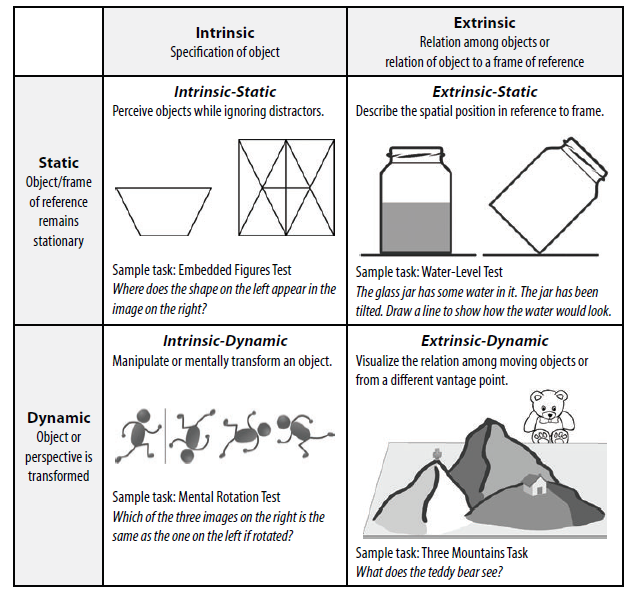
\includegraphics[width=\textwidth,height=\textheight,keepaspectratio]{fig_1-1}
   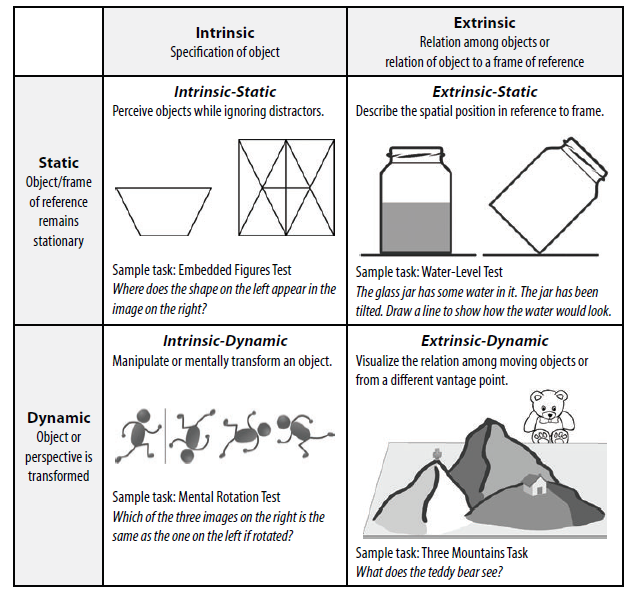
\includegraphics[scale=1]{fig_1-1}
   \caption[{2x2 topology of spatial reasoning categories}]{2x2 topology of spatial reasoning categories \parencite{davis2015spatial}.}
   \label{fig:fig_2-1}
\end{figure}


\subsect{Development of Spatial Reasoning in Early Years}
Development of spatial reasoning starts in early years of human life. Different researchers have presented their theories about timeline of development of spatial reasoning skills in children \parencite{yilmaz2017development}. Piaget and Inhelder \parencite{piaget1956child} indicated that children go through three stages during this development of their cognitive spatial ability: preoperational stage, concrete operational stage and formal operational stage. They indicated that children under six years of age can locate objects with respect to themselves and are aware of topological spatial relationships. They are in preoperational stage since they understand concepts like separation, proximity and open/close. In concrete operational stage, children of ages 7-9 years develop a cognitive map with a fixed frame of reference helping them with external view and orientation such as right/left and before/behind. At age of 11, as children enter the last stage i.e., formal operational stage, they understand concept of fixed positions relative to each other that assist them in understanding concepts such as proportional reduction of scale, and estimating straight-line relative distances. \\
However, later around 2000, Huttenlocher and Newcombe \parencite{huttenlocher1999spatial} suggest that spatial reasoning develops even earlier, as early as at age of 6 months. Stages presented by them are summarized as follows \parencite{yilmaz2017development}: 
\begin{enumerate}
    \item Infants at age of 6 months are able to use dead reckoning skills to understand location of objects around. This helps them in keeping track of moving object's direction.
    \item At age of 12 months, babies can find hidden stimuli with help of understanding of distance.
    \item At age of 18 months, they can navigate easy routes.
    \item Using the distance information from landmarks, kids can define locations at age of 2 years. Piaget had suggested that does not happen until they are nine or ten. 
    \item Kids at age of 3 are able to use simple maps and models.
    \item If encouraged to play with maps and tools, kids can fully develop their spatial reasoning skills by the age of nine or ten. 
\end{enumerate}
Frick and Wang \parencite{frick2010round} experiments suggest that 14 month olds with some prior experience can activate mental rotation ability. Younger kids manifest the spatial reasoning skills which can be channeled by mental rotation exercises at early age to further strengthen this ability. However, at this young age, children can only continue an already started rotation.\\
Research on spatial transformations has indicated complex tasks like mental paper folding task emerges at age of 5.5 years and continue to improve through early elementary school \parencite{harris2013new}. Object based spatial transformations require children to posses spatial manipulation ability of mental imagery. This occurs for kids aged between 7 and 8 years. Egocentric perspective transformations develop later at age of 8 years rather than 7, than object-based transformations \parencite{crescentini2014mental}. 

\subsect{Role of Spatial Reasoning in Mathematics}
Over 60 years ago, a report of a National Science Foundation (NSF) advisory panel, Scientific Careers, was published \parencite{super1957scientific} which emphasized on critical role of spatial ability. It was characterized as an individual difference that affected learning the advanced scientific-technical concepts for outstanding performance in STEM (science, technology, engineering and mathematics).Despite that this fact was established as early as 1957, spatial reasoning skills are not included in curriculum and instruction in educational settings even in STEM domains. Various studies and projects followed further solidifying the positive effect of spatial reasoning skills on success in STEM fields \parencite{wai2009spatial}. \\

There are several theories of quantitative reasoning on how spatial reasoning skills may support success in mathematics. Dehaene and his colleagues suggests that quantitative reasoning comprises of two core systems of numbers which tap different neural networks in the human brain: one being approximate and non-symbolic and the other is precise and symbolic. It is suggested that the first core shares neural activity with spatial reasoning skills and the second core is more associated with exact counting and symbolic mathematical operations \parencite{feigenson2004core}. As early schooling results in the two core systems of numbers merging, spatial skills' impact on mathematics achievement via the second symbolic system of number will increase significantly. Symbolic and non-symbolic numerical thinking will mutually enhance one and other as these are taught over time \parencite{piazza2013education}. Existing evidence suggests that the spatial skills, if polished in early elementary school curriculum, will provide a strong foundation for mathematics achievement in elementary school and beyond. \\
Various studies imply that in elementary school students, spatial skills are known to support understanding of geometry \parencite{clements1997development},  word problem solving and application of more complex and complicated computation strategies \parencite{manger1998effects}, especially in girls \parencite{dearing2012young}. Longitudinal studies have also shown that early spatial skills predict later success in mathematics. For instance, spatial reasoning skills measured in first-grade girls are crucial predictors of fifth-grade analytical math reasoning.  First-grade assessments included spatial skills, verbal skills, addition/subtraction skills, and frequency of choice of a decomposition or retrieval strategy on the addition/subtraction problems. In fifth grade, girls were given an arithmetic fluency test, a mental rotation spatial task, and a numeric and algebra math reasoning test \parencite{casey2017girls}. Similarly, spatial visualization predicted as early as in kindergarten reflects arithmetic skills in third graders. Linguistic and spatial skills can improve arithmetic development by enhancing children's number‐related knowledge \parencite{zhang2014linguistic}. Even at early ages, both mental rotation and spatial visualization skills have depicted associations with numeric operations and  addition and subtraction computational skills in grade 1,2,3 and even in kindergarten. A 32-week-teacher-led spatial reasoning intervention in K-2 classrooms highlighted the importance of assisting development of spatial visualization in young kids as part of early mathematics instruction \parencite{Hawes2017}. Another longitudinal study investigated the development of spatial reasoning skills in 304 elementary school children as they progressed from grade 2 to 4 which outlines effects of socioeconomic status, verbal working memory and gender \parencite{carr2018development}. \\
To summarize, spatial reasoning skills contribute positively to development of mathematical understanding at early ages and are pertinent to achievements in STEM fields later on. 

\subsect{Ways to Augment Spatial Reasoning}
Spatial reasoning can be augmented using various activities and games. Following are some ways suggested to improve spatial skills:
\begin{enumerate}
    \item Use spatial language and gestures in everyday instructions: Using spatial language such as inside, outside, left, right, behind and on top of, assists babies in learning spatial relations better \parencite{casasola2008development}. For example, sentences to describe scenes: The car is across the street under the tree. Asking kids to repeat after you helps further. Hand-gestures along with spatial language can help kids learn better \parencite{singer2005children}.
    \item Teach how to visualize using mind's eye: Visualization is an essential tool for spatial learning. If kids are instructed to visualize a problem while solving it, they would perform much better. For instance, in an experiment, when a ball is dropped even through a twisted tube, preschooler would tend to think it falls right under. But when young kids are distracted from their gravity bias by instructing them to visualize the path of the ball, more students get the right answer \parencite{joh2011imagining}.
    \item Two-dimensional Puzzles and other activities: Various puzzles and matching games can be used to enhance spatial reasoning skills of kids. For instance, tangram, an ancient Chinese puzzle that consists of 7 pieces and can be rearranged into many different shape can help increase spatial skills of students \parencite{siew2013facilitating}.  Similarly, jigsaw puzzle, origami, paper folding, and other open-ended puzzles can help augment spatial visualization skills of kids as these require mental manipulation of various shapes. 
    \item Three-dimensional block play: Building structures and objects with 3D blocks e.g., Lego\textsuperscript\textregistered{} \parencite{wolfgang2003advanced} and wooden blocks can significantly increase children's ability to manipulate things mentally. Giving them a structure to build will expand their knowledge of spatial visualization. Block play is important in early years in helping kids understand spatial reasoning skills which are important for later STEM learning. When kids are prompted and asked questions about their block play structures by teachers or helpers, it grows their use of spatial language as well which is related to increase in spatial reasoning \parencite{pruden2011children} and can play an important role in scaffolding children’s building of more complex structures \parencite{kersh2008research}. A planned block play program similar to Carol Stephenson can help greatly in developing spatial reasoning skills through building complex block structures \parencite{tepylo2015developmental}. A study examining children's puzzle play \parencite{levine2012early} shows that it predicts children's later performance on a spatial transformation task. It also discusses how early puzzle play varies across children and engagement is associated with demographic variables as well as levels of parent language input.
    %% https://www.parentingforbrain.com/visual-spatial-reasoning-skills-stem/#improve
\end{enumerate}
For the sake of this research, we explored 3D block building as the way to augment spatial visualization that we experiment with in our system since 3D block building tasks is a multi-step complex process that involves spatial visualization, mental rotation and perspective taking skills.


% New section
\sect{Child-Robot Tutoring}
Social robots have made their way in educational setting for children in recent years. Research community has been focused on various aspects of social robots in education. Benefits of social robots, technical challenges for building robot tutors, their efficacy, impact of their appearance, role and their behaviour has been vastly studied \parencite{belpaeme2018social}. Application of social robotics in education has become popular because of availability of robust platforms, mature technology to the point that meaningful interactions using language and nonverbal behaviour are possible, and the established fact that embodiment results in higher learning gains in educational settings. In various educational settings embodiment of a robot plays an important role on improving the children's performance, engagement and motivation \parencite{kose2015effect} \parencite{kennedy2015comparing}. Many aspects of child-robot tutoring has been investigates such as building models of student knowledge \parencite{spaulding2016affect}, evaluating different teaching and instruction paradigms \parencite{hood2015children}, personalizing content for each child \parencite{gordon2016affective} and determining when and how to provide specific kind of assistance and hints \parencite{ramachandran2016shaping}. Much of work in which robot is used as a tutor focuses on one-on-one interactions because these offer the greatest potential for personalization \parencite{belpaeme2018social} \parencite{ramachandran2019personalized}. Most of the research has focused on teaching languages \parencite{gordon2016affective} and solving mathematical problems \parencite{ramachandran2019personalized}. 


\subsect{Child-Robot Tutoring and Spatial Reasoning}
Spatial reasoning is rather unexplored in one-on-one child-robot tutoring. Reasons can be complexity of interaction, lack of ways to track performance and measure learning gains during complex tasks and difficulty in providing appropriate feedback. However, over the past two decades computer-supported educational tools are being used in learning of spatial skills particularly reflected in geometry e.g., Edwards created a computer environment that enabled kids to learn introductory geometric transformations \parencite{edwards1991children}. GeoCAL \parencite{chang2007developing}, a multimedia learning software based on van Hiele's theory of geometric thinking \parencite{chang2007developing} comprising of several games such as jigsaw puzzles, shape tracer and stamping, has notable learning effects on geometric thinking (visual association, description and abstraction). \\
However, models designed to improve spatial ability in 2D world by using Web-based virtual environment \parencite{rafi2005improving}  may not work at all in 3D world because of over-simplification of the environment. Therefore, Keren et al. 
\parencite{keren2012kindergarten} suggested that spatial cognition models should at least be partially embodied and assistive robots can serve the purpose in developing children's visual-spatial and motor perception. They use assistive robots for groups (2-3 kids) of kindergarten students to promote their geometrical thinking which is one aspect of spatial cognition. The activity for this study is modification of their previous research i.e., Nao (the robot) singing the Hebrew version of song, "Head, Shoulders, Knees and Toes" while demonstrating the movements and invited kids to do some movements \parencite{fridin2014robotics}. In this study, robot asks to recognize basic shapes on screen and distinguish between upper and lower parts of its body and are asked to find and push relevant buttons. \\
To summarize, development of spatial reasoning specially spatial visualization skills in 3D environment using educational social robotics is limited and rather unexplored. Thus, in this exploratory study we focus on providing a learning platform comprising of a robot tutor to help learn spatial visualization skills using 3D block building. We track the performance of children and assist them in completing a structure building task in one-on-one child-robot tutoring session.     

\sect{Feedback Strategies}
Good feedback practices by tutors in one-on-one sessions are essential for self-regulated learning. Good feedback practice is broadly defined as something that reinforces the student's capability to self-regulate their own performance. Self-efficacy in turn has positive effects on not only achievement, but also motivational variables such as engagement, effort and persistence \parencite{narciss2004impact}. For designing a good feedback practice, one needs to consider many factors. One of many principles to think about design and evaluation of self-created feedback procedures, is that feedback can be provided by a teacher, peer or tutor. Seven principles to think about design and evaluation of self-created feedback procedures are described below \parencite{nicol2006formative}: 
Good feedback practice: 
\begin{enumerate}
    \item helps clarify what good performance is (goals, criteria, expected standards)
    \item facilitates the development of self-assessment (reflection) in learning
    \item delivers high quality information to students about their learning
    \item encourages teacher and peer dialogue around learning;
    \item  encourages positive motivational beliefs and self-esteem
    \item provides opportunities to close the gap between current and desired performance
    \item  provides information to teachers that can be used to help shape teaching
\end{enumerate}
Informative tutoring feedback provides useful information strategically for task completion rather than offering complete solution. Interactive-Tutoring-Feedback (ITF) refers to feedback components to guide the student toward successful task completion. Narciss has proposed the ITF model that encapsulated the state of the art in developing feedback strategies for interactive learning tasks \parencite{narciss2005informatives} \parencite{narciss2008feedback} \parencite{narciss2013designing}. As per this ITF model, a feedback strategy is defined as a coordinated plan integrating clear and decisive statements specifying at least the following aspects of a learning process with feedback \parencite{narciss2012feedback}:
\begin{enumerate}
    \item \textit{scope and function}: what goals or purposes the feedback serves.
    \item \textit{content}: what information is given through the feedback.
    \item \textit{presentation}: in which form and modes the feedback content is given.
    \item \textit{conditions}: under which situational or individual conditions the feedback is provided.
    \item \textit{timing and schedule}: which event within the learning process trigger feedback statements. 
\end{enumerate}
This definition enables a wide range of possibilities when it comes to designing feedback strategies. Feedback comes in various forms and modes i.e., immediate vs. delayed feedback timing, single-try vs multiple-try, adaptive vs non-adaptive and implicit vs explicit feedback \parencite{narciss2008feedback}. In human-human interactions, experienced tutors tend to provide indirect feedback to bring the attention of students to an error rather than giving corrective explicit feedback \parencite{lepper1990self}. Indirect corrective feedback is argued to address some of weakness of direct corrective feedback (CF) (e.g., no explanation to why the correction is needed), as indirect CF engages learners to analyze their own work and figure out and correct their mistakes Expert tutors also employ subtle techniques like delaying affirmation or expressing short hesitation when student inquires if he is doing alright, thus, hinting him about a mistake in the current step \parencite{fox1991cognitive}. There are other strategies like asking a leading question or subtly suggesting the student to redirect. Such strategies are enlisted in Table \ref{tab:tab_2-1}. On the other hand, it is argued that providing only implicit feedback can be detrimental. If a student spends too much time guessing for a solution or redirecting himself, it would be difficult for him to trace the path he took to solution \parencite{lewis1985discrimination}. Therefore, the tutoring strategy might be considered a trade-off between implicit and explicit feedback to allow room for the student to explore and learn from his mistakes, yet not be confused or stuck at an impasse. 



Kleij et al. \parencite{van2015effects} present a meta-analysis of effects of feedback on  student's learning outcomes in computer-based learning environments. They deduce that elaborated feedback is particularly more effective than feedback regarding correctness of answer and providing correct answer, specially in mathematics. The results suggested that immediate feedback is better for lower order learning than delayed feedback, whereas delayed feedback is more effective for high order learning. In the literature, there are contradicting results about effectiveness of immediate and delayed feedback. It seems to be task dependent. Thus, in this exploratory study we focus on providing direct/explicit or indirect/implicit feedback as soon as a mistake is made. We also provide confirmations on correct actions of user.  


\begin{longtable}{ | m{30em} | m{2cm}|  } 
\hline
\textbf{Feedback Strategy} & \textbf{Reference}  \\ 
\hline
1. Draw student’s attention to an error and provide second chance & \parencite{lepper1990self}  \\ 
\hline
2. Frequent feedback: Brief agreement with each step (e.g., Mhm and Right) when student is thinking out loud looking for agreement) or a short hesitation (often less than 1 sec) in responding with an “okay” indicating to students to assume that something was amiss with the current step & page 9,10 of \parencite{fox1991cognitive}  \\ 
\hline
3. Asking a leading question/ giving clues & \parencite{fox1991cognitive}\\
\hline
4. Asking a leading question/ giving clues.  Wait for student to complete your utterance, if student fails, complete it. Both work to avert a wrong solution & \parencite{lepper1990self}\\
\hline
5. Procedural hints and explanations: procedural hints point out appropriate strategy or mention key aspect of underlying concepts (e.g,. \emph{When expanding a fraction, one alters the numerator and denominator equally}). While procedural explanations provide more details about how to put this procedure into practice. (e.g., \emph{When expanding a fraction, one alters the numerator and denominator equally. To do this, multiply the numerator and denominator by the same number.}). & \parencite{narciss2014exploring}\\
\hline
6. Conceptual hints and explanations: focus on conceptual knowledge important for solving the target problem e.g., conceptual hint: \emph{When expanding a fraction, its value must not change.} and conceptual explanation: \emph{When expanding a fraction, its value must not change. While expanding, the denominator increases, that means the partitioning becomes more fine-grained. But since the value of the whole fraction does not change, the numerator has to be altered in the same way}. Conceptual explanations provide additional information about relevancy of the concepts to the given problem. & \parencite{narciss2014exploring} \\
\hline
7. Feedback consists of following components: & \parencite{parvez2008individualizing}\\
a. Definition: verbally introduce definitions of domain concepts e.g., \emph{Attributes are characteristics of an object that persist through the life of the object.}. & \\
b. Example: give an illustration of given concept e.g., \emph{Attributes of a car might be its color, model and make} & \\
c. Question: ask a question for clarity of learner e.g., \emph{Why did you set the data type for money to string?} & \\
d. Scaffold: prompts the learner who might be lost towards a correct solution by pointing in right direction e.g., \emph{Use the tutorial to learn about datatypes.} & \\
e. Picture: contains images, animation or video to visually explain a concept. & \\
f. Relationships: provides information to help learner understand how a concept fits into the overall problem solving activity. & \\
g. Application: shows application of a concept e.g., a learner might know definition of a constructor but might not know that a class could have multiple constructors. & \\
h. Exercise: supports active learning through hands-on activities or by applying a concept. It is more like a tutorial mode. & \\
\hline
8. Corrective feedback have been classified into two groups for second language teaching: & \parencite{ferreira2007study} \\
a. Giving-Answer Strategies (GAS): when teacher directly gives the target form or shows the location of student's error. These includes: repetition, recast, explicit correction and giving answer. &\\
b. Prompting-Answer Strategies (PAS): when teacher pushes students to notice their error and correct it themselves. These include: Meta-linguistic cues (teacher provides information or asks questions regarding the correctness of the student's utterance), clarification requests and elicitation(allowing student to complete teacher's utterance and by asking student to reformulate the utterance). & \\
\hline
\caption[Feedback strategies from the literature]{Feedback strategies from the literature.}
\label{tab:tab_2-1}

\end{longtable}

